\chapter{Literature Review}\label{LiteratureReview}
For this dissertation, research was conducted to identify the most recent trends in 2D fluid segmentation of OCT volumes using deep learning, as well as the application of generative models for intermediate slice synthesis.
\section{Fluid Segmentation in OCT Scans}
In the fluid segmentation state-of-the-art research, articles were retrieved using a systematic review methodology. The next subsection details the retrieval process and the criteria for inclusion and exclusion of the articles. Section \ref{FluidSegmentationLiteratureReview} presents the trends in methodologies used for fluid segmentation.
\subsection{Search Strategy}\label{SearchStrategy}
The search query was defined as: ````OCT'' AND ``segmentation'' AND (``deep learning'' OR ``CNN'' OR ``neural network'')''. Using the query, papers were retrieved from four different databases: 398 articles from PubMed, 105 from IEEE, 125 from ScienceDirect, and 80 from ACM.
\par
In the process of collecting the papers, those published over the previous five years and regarding 2D or 2.5D fluid segmentation in OCT volumes were included. Additionally, conference proceedings, non-English articles, and articles without the full text accessible were excluded.
\par
A total of 708 articles were initially identified, of which 133 were duplicates. Afterwards, 575 articles were screened, based on titles and abstracts. These articles were analyzed in accordance with the inclusion and exclusion criteria, resulting in the removal of 499 papers. Of the remaining 76 articles for the full-text screening, 20 met the established criteria. These final articles represent the state-of-the-art in 2D deep learning-based fluid segmentation in OCT volumes included and form the foundation of the literature reviewed in this dissertation.

\subsection{Trends in Segmentation Methodologies}\label{FluidSegmentationLiteratureReview}
The selected papers can be divided into two broad groups, according to the type of segmentation: binary segmentation \parencite{Quek2022, Pawan2021, Liu2021, Guo2020, Wang2021, Wu2023}, where the fluid is classified in one whole class, and multi-class segmentation \parencite{Rahil2023, Hassan2021a, Zhang2023, Sappa2021, Xing2022, Tang2022, Padilla2022, Hu2019, Mantel2021, Liu2024, Li2023, Gao2019, Hassan2021b, Lu2019}, where the segmented fluid is classified in two or more classes (namely IRF, SRF, and PED). Additional grouping criteria include the segmentation architecture and the use of retinal delimitation, as shown in Figure \ref{fig:ArticlesSelection}.
\par
In binary segmentation, the approaches to the segmentation problem are simpler, but include both convolutional neural networks (CNN) \parencite{Pawan2021, Liu2021, Guo2020, Wang2021, Wu2023} and transformer solutions \parencite{Quek2022}. The CNN solutions differ among them, depending on the modules that constitute each network, but all are inspired by the U-Net \parencite{Ronneberger2015}. In Figure \ref{fig:BinarySegmentationExample}, an instance of a CNN used for binary fluid segmentation is shown.
\begin{figure}[!ht]
	\centering
	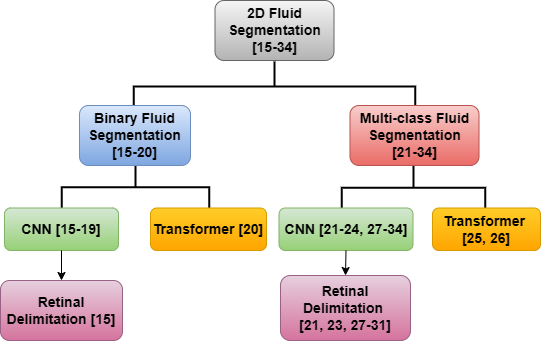
\includegraphics[width=0.75\linewidth]{figures/ArticlesSelection.png}
	\caption{Grouping of the articles included in the literature review.}
	\label{fig:ArticlesSelection}
\end{figure}
\begin{figure}[!ht]
	\centering
	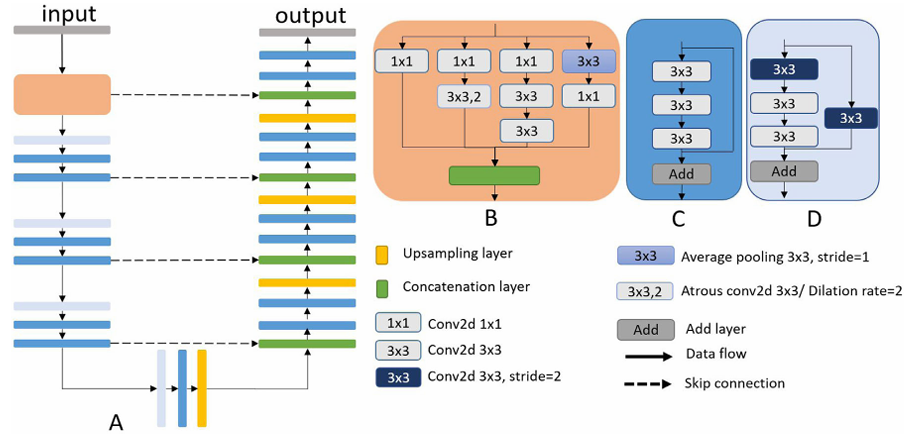
\includegraphics[width=1\linewidth]{figures/BinarySegmentationExample.png}
	\caption{Example of a CNN architecture used for binary fluid segmentation. Image A depicts the neural network architecture, B shows the used multi-scale block, while C and D exhibit the residual convolutional blocks \parencite{Guo2020}.}
	\label{fig:BinarySegmentationExample}
\end{figure}
\par
The work of \textcite{Pawan2021} is the only one in binary segmentation that restricts the input of the CNN to the content within the retinal layer. This approach is frequently observed in the papers focused on multi-class segmentation. In \parencite{Pawan2021}, this is achieved by performing a retinal layer segmentation and assigning all the values outside the boundaries to zero. The result of this operation serves as input to the CNN. The removal of irrelevant information surrounding the retina simplifies the learning process and improves the model's focus on essential information \parencite{Mantel2021}.
\par
In the framework proposed by \textcite{Liu2021}, the  slice's fluid mask and distance map are generated. The distance map consists of the predicted distance of each pixel to the retinal tissue, with only the values above a specified distance threshold being kept. This is achieved through the use of a double-branched network, where the encoder is the same, while the decoders vary. One decoder is responsible for generating the fluid segmentation map, while the other predicts the distance map. This distance map is then converted to a binary mask by applying a threshold value: pixels with greater distance than this value are set to one, and all others to zero. The intersection between the fluid segmentation map and this binary mask forms the final segmentation. This approach mitigates the issue of inappropriate merging of small and proximate fluid regions, as the distance map branch is better than the fluid segmentation network in discerning the boundaries that delineate fluid regions.
\par
Resorting to generative adversarial networks (GANs), \textcite{Wu2023} make images from different vendors visually similar to the images of a singular, specific vendor. Subsequently, a U-Net, which has extensively been trained on images from that specific vendor, is used for segmentation. This approach is intended to reduce the burden of learning the segmentation on multiple vendors by ensuring that all volumes are similar to one in which the segmentation model performs well. The multi-class segmentation framework proposed by \textcite{Li2023} was designed based on the same idea. 
\par
CNNs inspired by the U-Net can also be combined with transformers in the context of binary fluid segmentation \parencite{Quek2022}. While CNNs capture the information from local receptive fields, visual transformers integrate features from global receptive fields. In the neural network proposed by \textcite{Quek2022}, the visual transformers are located between the encoder and decoder paths, thus incorporating features from both receptive fields in the encoding branch.
\par
The majority of the papers included in this review perform multi-class segmentation, which results in a broader range of implementation strategies. While all of them segment two or more types of fluids, \textcite{Hassan2021a} and \textcite{Padilla2022} also segment other retinal biomarkers. Similarly to binary segmentation, the multi-class segmentation papers can also be divided according to the presence \parencite{Zhang2023, Liu2024} or absence \parencite{Rahil2023, Hassan2021a, Sappa2021, Xing2022, Tang2022, Padilla2022, Hu2019, Mantel2021, Li2023, Gao2019, Hassan2021b, Lu2019} of transformers in the segmentation network. All the papers that have transformers in their framework combine them with CNNs. 
\par
Similar to what was developed by \textcite{Quek2022}, \textcite{Liu2024} have integrated transformers in the bottleneck section of a segmentation network inspired by the U-Net. The authors utilize two networks for the segmentation: one for coarse segmentation and other for the refinement of the results from the first. Both networks are similar to the U-Net, but a transformer is included in the refinement branch. Its purpose is to provide features from global fields, compensating for the deep features that are used as input in this branch. In contrast, \textcite{Zhang2023} replaced the CNN encoder with a transformer encoder, exploiting its modeling capacity with self-attention.
\par
The limitation of the input to the region within the retinal layer, ignoring what is outside of it, is seen in many of the multi-class papers \parencite{Hassan2021b, Hassan2021a, Lu2019, Mantel2021, Rahil2023, Tang2022, Xing2022}, similarly to what was done in \textcite{Pawan2021}. There are various approaches for this delimitation, with some using CNNs trained for the segmentation of the retinal layers or the retina \parencite{Mantel2021, Tang2022}, and others relying on algorithms that detect the distinct transition in intensity or texture between the retina and the surrounding tissue or background \parencite{Hassan2021b, Hassan2021a, Lu2019, Rahil2023, Xing2022, Pawan2021}. 
\par
The retinal delimitation is conducted as a separate process from the fluid segmentation. In \parencite{Tang2022, Hassan2021b, Hassan2021a, Lu2019, Rahil2023, Xing2022}, the retinal layer is segmented prior to the fluid segmentation, conditioning the input of the fluid segmentation network and simplifying the learning process. However, the retinal delimitation can also constrain the final output by limiting segmentation to the retinal layer zone, as observed in \textcite{Mantel2021}.
\par
The input can be conditioned in multiple ways. \textcite{Xing2022} crop the image to fit the region of interest. In \parencite{Rahil2023, Tang2022, Lu2019}, the OCT B-scan is combined with the retinal delimitation result through concatenation. Conversely, in \parencite{Hassan2021b, Hassan2021a, Pawan2021} the information outside the retinal layer is set to zero and ignored. 
\par
Contrasting with the work of \textcite{Liu2021} who used a CNN for returning a distance map (relative to the retinal tissue), \textcite{Tang2022} and \textcite{Rahil2023}, inspired by the work of \textcite{Lu2019}, calculate a relative distance map to the internal limiting membrane (ILM), which is concatenated with the input B-scan in a CNN. Starting with the retinal delimitation, the relative distance to the ILM is calculated for each pixel located between the ILM and the Bruch's membrane (BM) (see Figure \ref{fig:RetinalLayers}). This map provides information about each pixel's relative position to the ILM, influencing their classification. An example of such framework can be seen in Figure \ref{fig:PreSegmentationAndFluidSegmentation}.
\par
\begin{figure}[!ht]
	\centering
	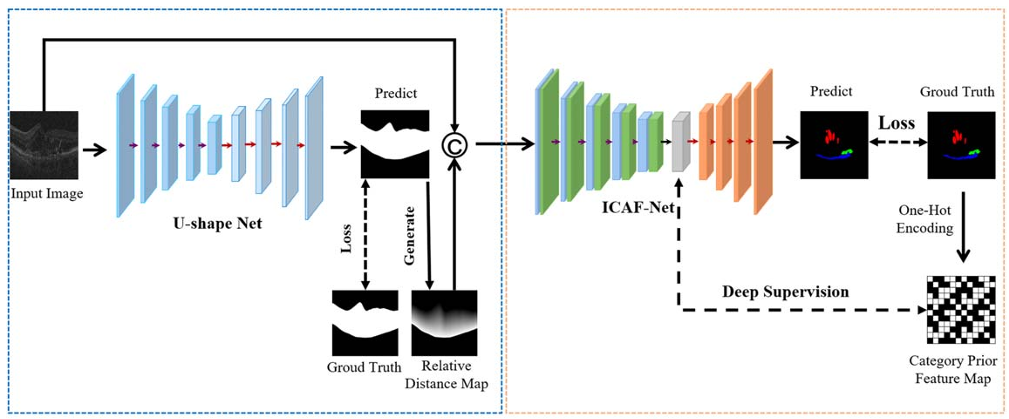
\includegraphics[width=1\linewidth]{figures/PreSegmentationAndFluidSegmentation.png}
	\caption{Example of a framework that includes retinal layer delimitation and construction of a relative distance map (left side). The generated map, together with the original image, serves as input to the segmentation network (denominated ICAF-Net, by the authors) \parencite{Tang2022}.}
	\label{fig:PreSegmentationAndFluidSegmentation}
\end{figure}
\par
Regarding the segmentation CNNs adopted by the analyzed papers, most are directly inspired by the U-Net, to which changes are done when considering the objectives of each study. Examples of such changes are the introduction of blocks (such as residual \parencite{Mantel2021, Zhang2023, Liu2024, Hassan2021b, Hassan2021a, Padilla2022}), and modules (like atrous sampling pyramid pooling \parencite{Hassan2021b, Hassan2021a, Hu2019, Sappa2021}), which makes the network distinctive. However, some papers use other variations of the U-Net that are also popular: the Deeplab \parencite{LChen2018} in \textcite{Hassan2021a, Li2023}, and the VGG \parencite{Simonyan2014} in \textcite{Padilla2022, Hassan2021b}.

\section{Intermediate Slice Synthesis}
For many years, there have been attempts to improve the resolution of OCT exams using computational methods, a process called super-resolution (SR). In 3D applications, such as magnetic resonance imaging (MRI), computed tomography (CT), and OCT, SR can be applied either intra-slice, improving the resolution of each slice in the volume along one plane, or inter-slice, enhancing the resolution of the volume along one axis by generating one or more slices between a pair of original ones. Some frameworks may even combine both approaches \parencite{You2020}.
\par
The use of GANs for generating slices between pre-existing slices is a commonly used technique in MRI and CT, but with few examples in OCT \parencite{You2020}. The systematic literature review performed by \textcite{Ibrahim2024}, which analyzed the latest trends in the use of generative models in medical data, only presents one example of GAN for inter-slice resolution improvement in OCT volumes \parencite{Lopez2023}. In this imaging technique, the use of GANs is mainly done for the generation of OCT images and conversion between different vendors \parencite{Ibrahim2024}.
\par
In the following subsection, the state-of-the-art architectures used for the improvement of inter-slice resolution are presented.

\subsection{Architectures for Medical Image Super-Resolution}
Given the lack of examples in OCT imaging, it was considered appropriate to study works from other imaging techniques, such as CT, MRI, and even video, given that the working principle is the same across them. The selected papers that are applied to medical images can be classified into three distinct categories: inter-slice SR, which leverages information from adjacent slices to generate one or more intermediate slices \parencite{Lopez2023, Xia2021, Wu2022, Nishimoto2024}; intra-slice SR combined with inter-slice SR, which improves the resolution of the slices from orthogonal planes and combines them with the results of inter-slice SR \parencite{Zhang2024, Peng2020, Fang2022, Nimitha2024, Georgescu2020}; and SR applied directly in 3D volumes, utilizing three-dimensional convolutions in the generation process, which incorporates the information along all the axes from multiple slices simultaneously \parencite{YChen2018, Sanchez2018, Kudo2019, Zhang2022}.
\par

\subsubsection{Inter-slice SR}

\textcite{Lopez2023} present an inter-slice SR framework based on a GAN, inspired by the ResNet, for the generation of three B-scan slices between two known slices. The GAN training process, as illustrated in Figure \ref{fig:GANGenerationFramework}, begins with the generation of an intermediate slice (Central Fake) located between two original B-scans (Pre and Post), which are separated by another original one (Central). The Central B-scan serves as the ground truth (GT) and is used in the assessment of the quality of the image generated by the network. Subsequently, the network generates other two slices: one between the Pre and Central slices, designated as Pre-Central fake, and another between the Central and Post slices, named Post-Central fake. Since these generated slices lack corresponding GT, the network's performance is regulated by using these two new synthetic slices for generating an additional intermediate slice (Central Fake 2), which is then compared to the true Central. Consequently, if the generation of Pre- and Post-Central fake images are inadequate, the Central Fake 2 will also be of poor quality, resulting in a higher loss value. During the inference process, one slice is synthesized for every two known B-scans, reducing the inter-slice distance to half of the original value.
\par
The importance of this study comes not only from it being the only study in OCT but also from the approach selected, which is similar to the foundation of the frameworks implemented in other papers. 

\begin{figure}[!ht]
	\centering
	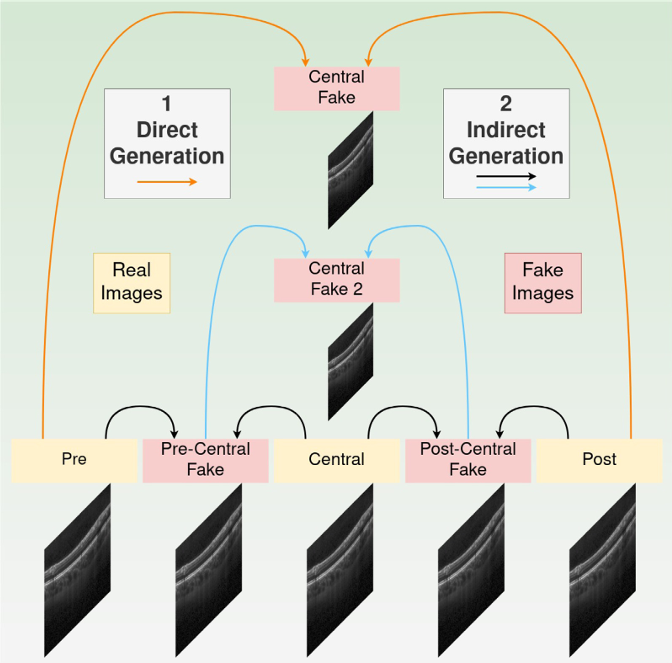
\includegraphics[width=0.70\linewidth]{figures/GANGenerationFramework.png}
	\caption{\textcite{Lopez2023} training process.}
	\label{fig:GANGenerationFramework}
\end{figure}

In a more straightforward approach, \textcite{Nishimoto2024} utilize a baseline U-Net that uses two spaced slices as input to generate the slices between them. This methodology was tested in the generation of three, four, and five intermediate slices, and obtained better outcomes than those generated through linear interpolation. This approach works particularly well due to the low noise present in the CT scans. In volumes with more noise, due to the presence of metal artifacts, the slices generated using the U-Net are of worse quality than those obtained through linear interpolation.
\par
The work by \textcite{Xia2021} demonstrates the enhancement of inter-slice resolution in MRI through the use of multiple networks and a multi-scale discriminator that considers both global and local features by processing different image scales and a scheme that illustrates this framework can be seen in Figure \ref{fig:XiaFramework}. The networks in this framework receive two slices ($x_{z\pm1}$) and generate a new one between them ($x_{z}$). The generator ($G$) is responsible for producing the intermediate slice, while the discriminator ($D$) learns to distinguish the synthesized image from the real image. The loss of these networks is also determined by the similarity of feature maps between images ($L_{FM}$).
\par
The framework contains two other U-shaped networks: one that learns to predict the optical flow and one that learns to predict the depth map for each input image. Based on the optical flow, depth maps, and their linear interpolation ($\bar{x_{z}}$), another U-shaped network generates the intermediate slice. The result from this network and the generator's output (to which Gaussian blurring is applied) are evaluated by the discriminator. Once again, the discriminator evaluates both images in separate feature spaces, processing each input at a different scale to extract both global and local representations for comparison.
\par
The image generated by the network using optical flow and depth ($\hat{x_{z}}$) pays special attention to the transitions between the two input slices. The point of inputting these images to the discriminator is to encourage it to recognize these characteristics in the generator's output. Additionally, the discriminator is exposed to blurred images to further incentive the generator to produce sharper images.

\begin{figure}[!ht]
	\hspace*{-0.35in}
	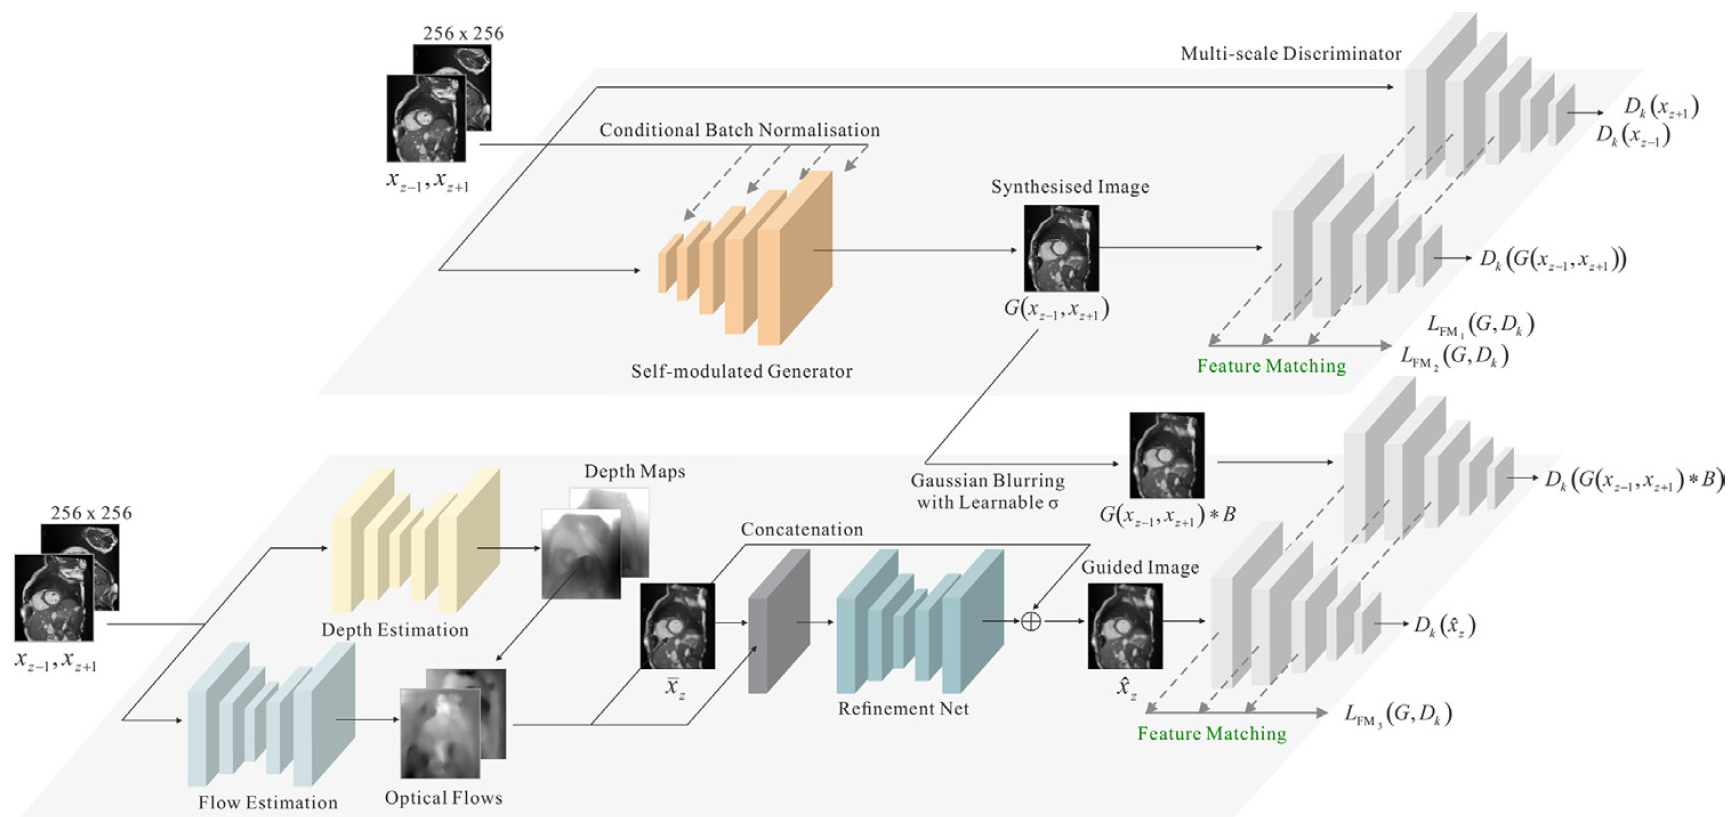
\includegraphics[width=1.1\linewidth]{figures/XiaFramework.png}
	\caption{Framework developed by \textcite{Xia2021}.}
	\label{fig:XiaFramework}
\end{figure}

\par
On the other hand, \textcite{Wu2022} improved the inter-slice resolution by training a generator network to output bi-directional spatial transformations instead of producing fake images. The advantage of this process is that it allows the same transformations to be applied to the segmentation masks from the surrounding slices, generating fake masks for the fake slices. 
\par
As in \textcite{Xia2021}, the GAN's discriminators also evaluate the generated images in both a larger and smaller field of view. To evaluate the output at a larger field of view, a global discriminator classifies the image as real or fake. Meanwhile, the evaluation at a smaller field of view integrates an attention network, which focuses on the most informative regions of the image to support the local discriminator and the object identifier. 
\par
The local discriminator classifies the image as real or fake based on fine-grained features extracted by the attention network. Meanwhile, the object classifier, which is a much shallower network, verifies whether certain structures present in the real image also appear in the fake one, using the output of the attention network. 
\par
By using both global and local discriminators, the generator is encouraged to output images that closely resemble the real images, both in the overall structure and fine details. The object detector ensures that the objects present in the real image are represented in the generated one.

\subsubsection{Intra- and Inter-slice SR}

As an example of combining intra-slice SR with inter-slice SR, \textcite{Zhang2024} implemented two networks that enhance the resolution of CT volume's slices in the two planes with the lowest in-slice resolution: sagittal and coronal. These networks increase the resolution only along the axial direction. The models here utilized are based on the anisotropic meta interpolation (AMI) network developed by \textcite{Peng2020}, a benchmark work in the field of medical image SR. 
\par
\textcite{Peng2020} introduced the AMI network as a single-image SR method designed to enhance the slice's resolution along the axis with the lowest spatial resolution - in this case, the axial axis. The AMI network is applied independently to the sagittal and coronal slices, generating complementary interpolations along the axial direction. A fusion network then combines these two outputs to synthesize high-resolution slices along the axial plane.
\par
The implementation by \textcite{Zhang2024} extends the use of the AMI network in the images of the sagittal and coronal planes by incorporating a GAN. This GAN takes two adjacent axial slices as input and generates an intermediate slice, with a framework that is similar to that of \textcite{Lopez2023}.
\par
The three networks are trained on downsampled CT scans from which every other axial slice is removed. The outputs of the sagittal and coronal AMI networks are compared to the corresponding slices in the original CT scans. Meanwhile, the GAN's output is compared to the GT axial slices from the original CT scan.
\par
Instead of using a dedicated fusion network as in \textcite{Peng2020}, \textcite{Zhang2024} introduce a loss function that directly compares the outputs of the AMI networks to the output of the GAN. This loss is backpropagated through the generator, encouraging it to output axial slices that are coherent with the content inferred by the AMI networks. This results in axial images that are not only visually consistent with the original CT slices but also integrate structural information from other anatomical planes. A scheme of this method is shown in Figure \ref{fig:ZhangFramework}.

\begin{figure}[!ht]
	\hspace*{-0.35in}
	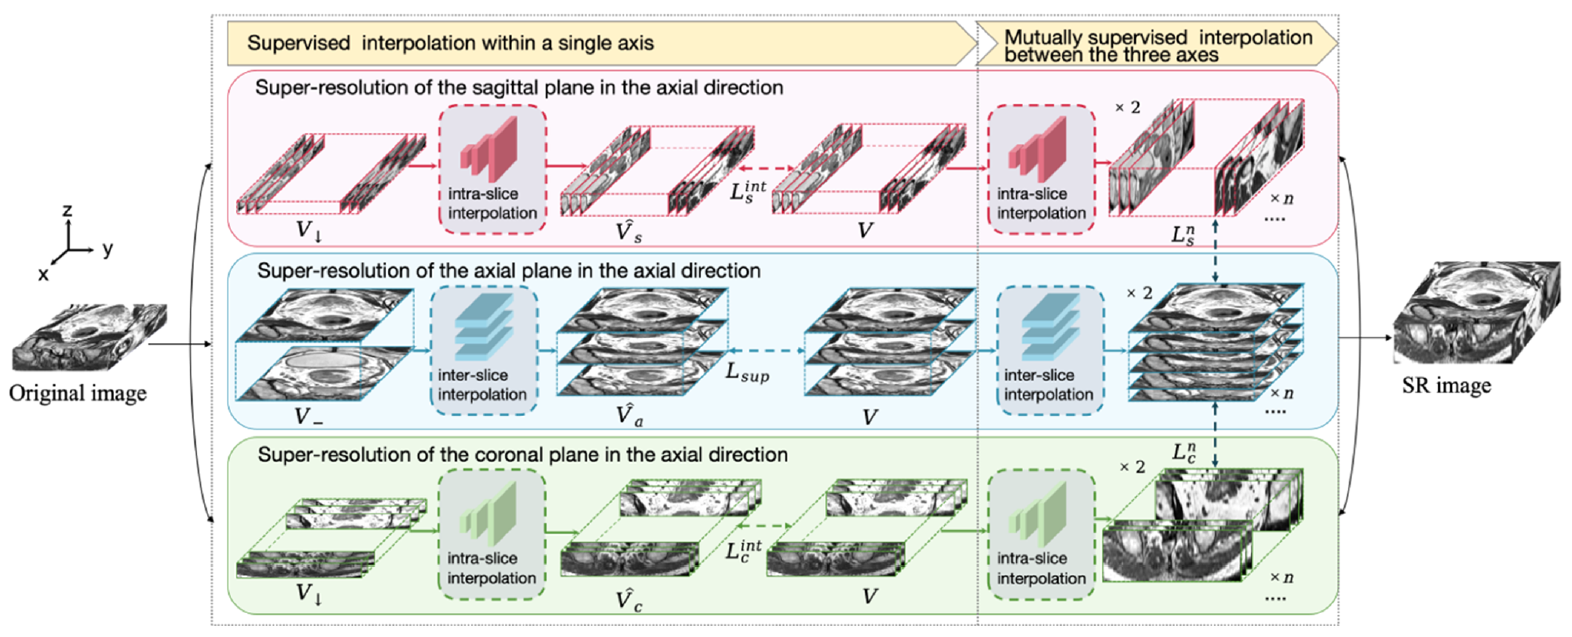
\includegraphics[width=1.1\linewidth]{figures/ZhangFramework.png}
	\caption{Architecture of the method developed by \textcite{Zhang2024}.}
	\label{fig:ZhangFramework}
\end{figure}

A similar approach was done by \textcite{Fang2022}. In this framework, three CNNs (one for each axis) are trained with the goal of generating the intermediate slices along the axis with a lower inter-slice resolution, which is the axial axis. Similarly to what is done in \textcite{Zhang2024}, two CNNs (one for the sagittal plane and one for the coronal plane) are trained to increase the resolution along the axial axis in the images of their respective plane. Both CNNs used in this work correspond to the single-image SR model developed by \textcite{Niu2020}. This CNN is an holistic attention network which improves the image's resolution by capturing both local and global contextual information. It uses holistic attention modules that combine channel attention (which emphasizes informative feature maps) and spatial attention (which highlights the most important regions of the image). This attention mechanism allows an image reconstruction with finer textures and sharper details in the super-resolved output.
\par
Instead of using a GAN to generate the intermediate slices along the axial plane, the authors apply another CNN. This network begins by extracting feature maps through space-to-depth transformation operations, which reorganize the spatial information into the channel dimension. The resulting features are then processed by a U-shaped architecture which captures both local and global context. Finally, a depth-to-space transformation is applied at the output layer, to reconstruct the intermediate axial slice at the original spatial resolution.
\par
All the networks are trained on downsampled CT volumes. After the first interpolation, all the outputs are compared to their respective GT and their loss is calculated. Then, another interpolation is performed in each axis, and a loss compares the generated images not with the GT, but with each other. This ensures coherence in the outputs predicted on different axis and transference of knowledge between them. During testing, inference is performed using a weighted prediction, with each axis' network contributing equally. In Figure \ref{fig:FangArchitecture}, the pipeline describing this implementation is shown.

\begin{figure}[!ht]
	\hspace*{-1.0in}
	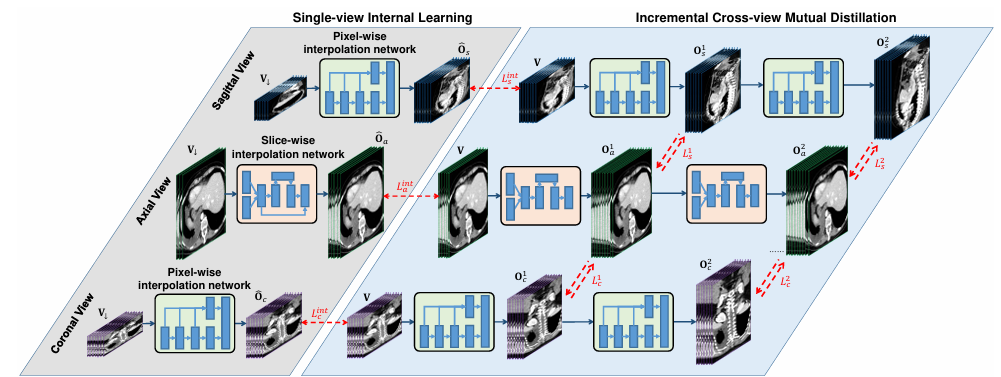
\includegraphics[width=1.25\linewidth]{figures/FangArchitecture.png}
	\caption{Pipeline of the methodology proposed by \textcite{Fang2022}.}
	\label{fig:FangArchitecture}
\end{figure}

\textcite{Nimitha2024} also perform intra-slice and inter-slice resolution enhancement. However, instead of improving both resolutions simultaneously as seen in \textcite{Zhang2024, Fang2022}, the enhancement is done sequentially. The pipeline starts with a low-resolution (LR), in which axial slices are firstly enhanced to becoming high-resolution (HR). Based on these HR axial slices, an intermediate slice is generated between each pair of consecutive axial slices.
\par
The network used in the enhancement of intra-slice resolution is a GAN. The generator starts with an in-plane and out-of-plane attention modules that extract features from the MRI slices adjacent to the target one. These extracted features are then passed through a U-shaped network that reconstructs the intermediate image. However, the number of upsampling blocks is higher than the number of downsampling blocks to ensure that the output has higher spatial resolution than the input.
\par
To generate the intermediate slices, the compression-driven frame interpolation (CDFI) network, a state-of-the-art video frame interpolation CNN developed by \textcite{Ding2021}, was utilized. CDFI is built on top of the AdaCoF module \parencite{Lee2020}, which is particularly powerful at handling a wide range of motions between images.
\par 
The CDFI network first extracts features using a U-Net architecture. These features are passed from the U-Net encoder to a pyramid network with the same number of levels as the encoder. At each level, a 1x1 convolution is applied to the feature maps to reduce dimensionality and prepare them for motion estimation.
\par
Two sub-networks take the U-Net's output and estimate the parameters of the AdaCoF operation. The U-Net's output is also combined with an occlusion mask to create the first candidate intermediate slice.
\par
The pyramid network's outputs are warped using AdaCoF and then passed into a synthesis network, which generates the second candidate intermediate slice. The two candidate intermediate slices are combined through a second occlusion mask to generate the final output. This model maintains visual realism from the first slice while ensuring a coherent pixel movement by using the second slice.
\par
\textcite{Georgescu2020} used a similar approach for enhancing intra- and inter-slice resolution in CT and MRI scans through two separate CNNs. One CNN was tasked with enhancing the resolution of the LR slices. Concurrently, the other CNN was utilized to reduce the distance between slices by increasing the resolution of the images from the orthogonal plane. By inferring an image with increased resolution along this plane, new intermediate slices were generated, improving the inter-slice resolution along the low resolution axis.
\par
The CNNs for intra- and inter-slice resolution are similar. Both networks consist of 10 consecutive convolutional layers, with the first 5 having 32 filters. The number of filters in the following layers changes according to the output size. This output size differs between the two CNNs because the first increases the resolution in two directions, while the other only increases the resolution in one direction.

\subsubsection{Three-dimensional SR}

The methodologies that use 3D GANs are similar to one another, as they all employ network architectures based on those used in 2D images. As the 3D GANs already considers the information across all the axes simultaneously, there is no need to use multiple networks for each, as seen in some of the previous approaches. Therefore, the differences between papers mainly originate from the medical imaging technique to which it is applied, the modules that constitute the 3D GANs used, and the datasets used for evaluation \parencite{YChen2018, Sanchez2018, Kudo2019, Zhang2022}.

\subsubsection{Video Frame Interpolation for Inter-slice SR in Medical Imaging}

Applications to increase the number of frames per second in a video work based on the same principle as the implementations that increase the inter-slice resolution of the three-dimensional volumes in medical images. In order to increase the number of frames in a video, these frameworks utilize two consecutive frames to generate an intermediate one, which is similar to what is seen in the previous papers that perform intermediate slice generation in medical images. The key difference between these applications is that, in video, the physical quantity that separates the frames is time, while the physical quantity that separates slices in medical imaging volumes is distance \parencite{Fang2022, Gambini2024}.
\par
Believing that the concepts that work on video also work on CT and MRI, \textcite{Gambini2024} implemented a state-of-the-art method of video interpolation to generate intermediate slices in CT and MRI. The method used was the real-time interpolation flow estimation (RIFE) \parencite{Huang2022}. The CNN incorporated in RIFE learns the pixel movements between frames from numerous examples. This approach, called contextual flow, appears as an alternative to optical flow - a method commonly utilized to describe the movement between frames which attempts to predict pixel movements by calculating their movement between consecutive frames. RIFE is also aware of the time difference between frames, which translates to the distance between slices in CT and MRI. To construct the middle image, the network learns how to blend the previous and following image so that the generated intermediate one looks more similar to the expected, combining it with the contextual flow. Lastly, a second network is used in the refinement of the generated image.
\par
Both networks learn based on a loss function that has three components: a photometric loss that determines how close the generated image is to the GT; a perceptual loss which evaluates the generated image as the human perception would; and a smoothness loss that evaluates how smooth the generated image is \parencite{Huang2022}.

\begin{figure}[!ht]
	\centering
	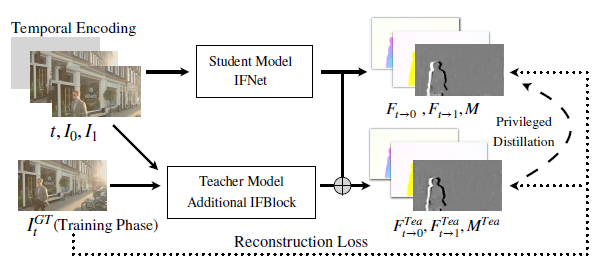
\includegraphics[width=0.85\linewidth]{figures/RIFEPipeline.png}
	\caption{Pipeline that describes the RIFE framework. The student model attempts to generate the intermediate frame, while the teacher refines the frame generated by the student so that it looks more similar to the middle frame. The results from both networks are evaluated on the reconstruction loss \parencite{Huang2022}.}
	\label{fig:RIFEPipeline}
\end{figure}

\textcite{Tran2020} present an alternative framework to the video frame interpolation. Instead of relying on contextual or optical flow to model pixel changes, two GANs are used for predicting the intermediate frame. The first generator receives as input the previous and following slice of the one desired to segment. The resulting slice is evaluated using the generator loss, which is composed of four components. This loss assesses how accurately the image is reconstructed and evaluates how well it fools the discriminator.
\par
The image resulting from the generator is given as input to the discriminator, which receives real and fake images as input and is responsible for correctly classifying it. The discriminator's prediction is compared to the true image's label, and the resulting loss is used in the adjustment of the discriminator weights.
\par
After training the first GAN, the second one is trained, which is a pix2pix \parencite{Isola2017}. Similar to what is seen in the work of \textcite{Gambini2024, Huang2022}, where a second network is used in the refinement of the output of the first one, this GAN is responsible for making the image output from the first GAN more similar to the original image. Contrasting with the previous examples where both the generative and refining networks are trained at the same time, the refining network is trained independently, after the training of the first network. The pipeline that describes this framework is shown in Figure \ref{fig:VideoGANFramework}.

\begin{figure}
	\centering
	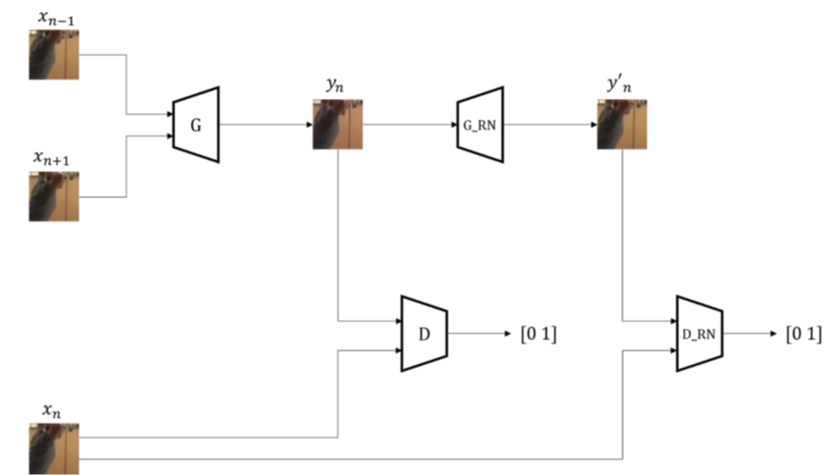
\includegraphics[width=1.0\linewidth]{figures/VideoGANFramework}
	\caption{Pipeline representing the framework developed by \textcite{Tran2020}. The generator that produces the intermediate frame is represented by $G$, while the discriminator is labeled $D$. The pix2pix generator is denoted by $G\_RN$ and the discriminator is represented by $D\_RN$. $x_{n-1}$ and $x_{n+1}$ respectively represent the previous and following frames of the one that is being generated, $x_{n}$. $y_{n}$ is the image generated by the first generator, while $y'_{n}$ is the image refined by the pix2pix network \parencite{Tran2020}.}
	\label{fig:VideoGANFramework}
\end{figure}
